% Created by tikzDevice version 0.12.3.1 on 2021-12-02 19:36:24
% !TEX encoding = UTF-8 Unicode
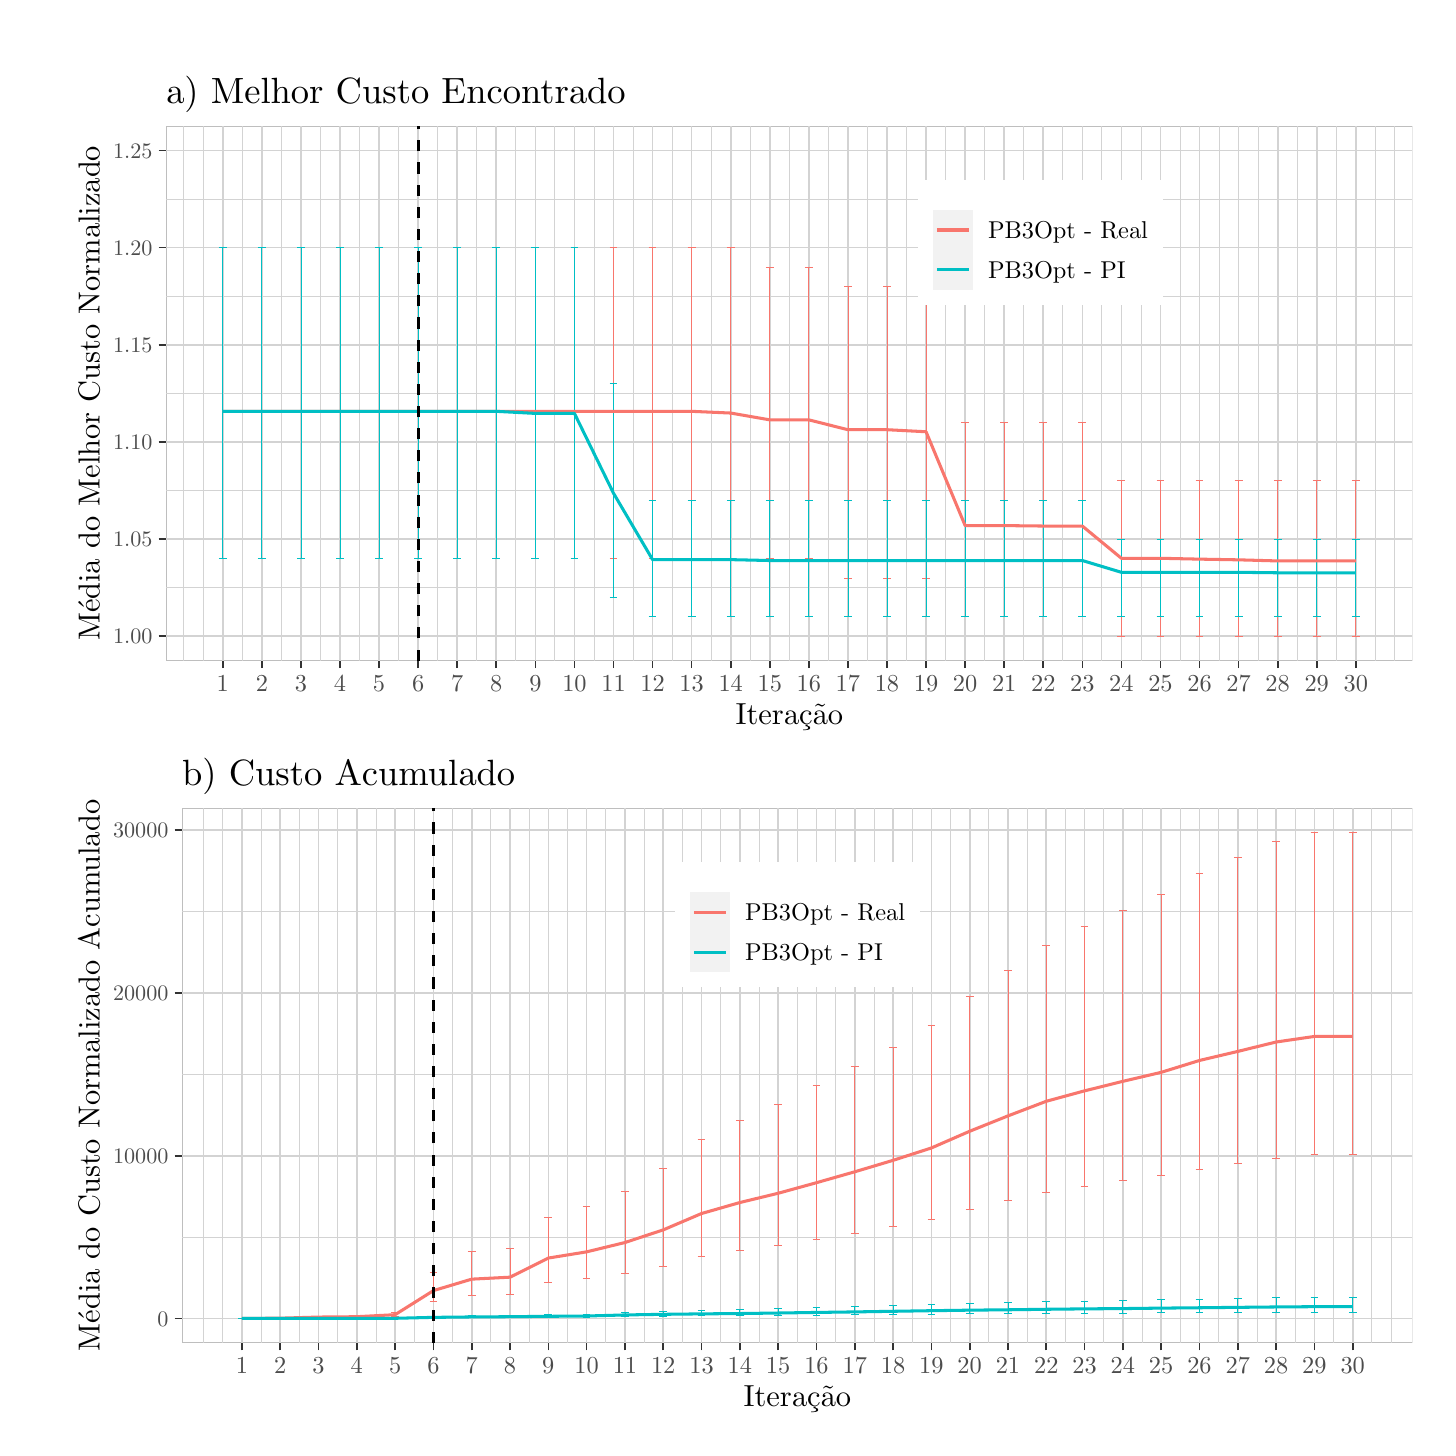
\begin{tikzpicture}[x=1pt,y=1pt]
\definecolor{fillColor}{RGB}{255,255,255}
\path[use as bounding box,fill=fillColor,fill opacity=0.00] (0,0) rectangle (505.89,505.89);
\begin{scope}
\path[clip] ( 12.91,246.49) rectangle (505.89,492.98);
\definecolor{drawColor}{RGB}{255,255,255}
\definecolor{fillColor}{RGB}{255,255,255}

\path[draw=drawColor,line width= 0.6pt,line join=round,line cap=round,fill=fillColor] ( 12.91,246.49) rectangle (505.89,492.98);
\end{scope}
\begin{scope}
\path[clip] ( 50.04,277.18) rectangle (500.39,470.32);
\definecolor{drawColor}{RGB}{190,190,190}
\definecolor{fillColor}{RGB}{255,255,255}

\path[draw=drawColor,line width= 0.6pt,line join=round,line cap=round,fill=fillColor] ( 50.04,277.18) rectangle (500.39,470.32);
\definecolor{drawColor}{RGB}{211,211,211}

\path[draw=drawColor,line width= 0.3pt,line join=round] ( 50.04,303.51) --
	(500.39,303.51);

\path[draw=drawColor,line width= 0.3pt,line join=round] ( 50.04,338.63) --
	(500.39,338.63);

\path[draw=drawColor,line width= 0.3pt,line join=round] ( 50.04,373.75) --
	(500.39,373.75);

\path[draw=drawColor,line width= 0.3pt,line join=round] ( 50.04,408.87) --
	(500.39,408.87);

\path[draw=drawColor,line width= 0.3pt,line join=round] ( 50.04,443.98) --
	(500.39,443.98);

\path[draw=drawColor,line width= 0.3pt,line join=round] ( 56.40,277.18) --
	( 56.40,470.32);

\path[draw=drawColor,line width= 0.3pt,line join=round] ( 63.45,277.18) --
	( 63.45,470.32);

\path[draw=drawColor,line width= 0.3pt,line join=round] ( 77.57,277.18) --
	( 77.57,470.32);

\path[draw=drawColor,line width= 0.3pt,line join=round] ( 91.69,277.18) --
	( 91.69,470.32);

\path[draw=drawColor,line width= 0.3pt,line join=round] (105.81,277.18) --
	(105.81,470.32);

\path[draw=drawColor,line width= 0.3pt,line join=round] (119.92,277.18) --
	(119.92,470.32);

\path[draw=drawColor,line width= 0.3pt,line join=round] (134.04,277.18) --
	(134.04,470.32);

\path[draw=drawColor,line width= 0.3pt,line join=round] (148.16,277.18) --
	(148.16,470.32);

\path[draw=drawColor,line width= 0.3pt,line join=round] (162.28,277.18) --
	(162.28,470.32);

\path[draw=drawColor,line width= 0.3pt,line join=round] (176.39,277.18) --
	(176.39,470.32);

\path[draw=drawColor,line width= 0.3pt,line join=round] (190.51,277.18) --
	(190.51,470.32);

\path[draw=drawColor,line width= 0.3pt,line join=round] (204.63,277.18) --
	(204.63,470.32);

\path[draw=drawColor,line width= 0.3pt,line join=round] (218.75,277.18) --
	(218.75,470.32);

\path[draw=drawColor,line width= 0.3pt,line join=round] (232.86,277.18) --
	(232.86,470.32);

\path[draw=drawColor,line width= 0.3pt,line join=round] (246.98,277.18) --
	(246.98,470.32);

\path[draw=drawColor,line width= 0.3pt,line join=round] (261.10,277.18) --
	(261.10,470.32);

\path[draw=drawColor,line width= 0.3pt,line join=round] (275.22,277.18) --
	(275.22,470.32);

\path[draw=drawColor,line width= 0.3pt,line join=round] (289.33,277.18) --
	(289.33,470.32);

\path[draw=drawColor,line width= 0.3pt,line join=round] (303.45,277.18) --
	(303.45,470.32);

\path[draw=drawColor,line width= 0.3pt,line join=round] (317.57,277.18) --
	(317.57,470.32);

\path[draw=drawColor,line width= 0.3pt,line join=round] (331.69,277.18) --
	(331.69,470.32);

\path[draw=drawColor,line width= 0.3pt,line join=round] (345.80,277.18) --
	(345.80,470.32);

\path[draw=drawColor,line width= 0.3pt,line join=round] (359.92,277.18) --
	(359.92,470.32);

\path[draw=drawColor,line width= 0.3pt,line join=round] (374.04,277.18) --
	(374.04,470.32);

\path[draw=drawColor,line width= 0.3pt,line join=round] (388.16,277.18) --
	(388.16,470.32);

\path[draw=drawColor,line width= 0.3pt,line join=round] (402.27,277.18) --
	(402.27,470.32);

\path[draw=drawColor,line width= 0.3pt,line join=round] (416.39,277.18) --
	(416.39,470.32);

\path[draw=drawColor,line width= 0.3pt,line join=round] (430.51,277.18) --
	(430.51,470.32);

\path[draw=drawColor,line width= 0.3pt,line join=round] (444.63,277.18) --
	(444.63,470.32);

\path[draw=drawColor,line width= 0.3pt,line join=round] (458.74,277.18) --
	(458.74,470.32);

\path[draw=drawColor,line width= 0.3pt,line join=round] (472.86,277.18) --
	(472.86,470.32);

\path[draw=drawColor,line width= 0.3pt,line join=round] (486.98,277.18) --
	(486.98,470.32);

\path[draw=drawColor,line width= 0.3pt,line join=round] (494.04,277.18) --
	(494.04,470.32);

\path[draw=drawColor,line width= 0.6pt,line join=round] ( 50.04,285.96) --
	(500.39,285.96);

\path[draw=drawColor,line width= 0.6pt,line join=round] ( 50.04,321.07) --
	(500.39,321.07);

\path[draw=drawColor,line width= 0.6pt,line join=round] ( 50.04,356.19) --
	(500.39,356.19);

\path[draw=drawColor,line width= 0.6pt,line join=round] ( 50.04,391.31) --
	(500.39,391.31);

\path[draw=drawColor,line width= 0.6pt,line join=round] ( 50.04,426.43) --
	(500.39,426.43);

\path[draw=drawColor,line width= 0.6pt,line join=round] ( 50.04,461.54) --
	(500.39,461.54);

\path[draw=drawColor,line width= 0.6pt,line join=round] ( 70.51,277.18) --
	( 70.51,470.32);

\path[draw=drawColor,line width= 0.6pt,line join=round] ( 84.63,277.18) --
	( 84.63,470.32);

\path[draw=drawColor,line width= 0.6pt,line join=round] ( 98.75,277.18) --
	( 98.75,470.32);

\path[draw=drawColor,line width= 0.6pt,line join=round] (112.87,277.18) --
	(112.87,470.32);

\path[draw=drawColor,line width= 0.6pt,line join=round] (126.98,277.18) --
	(126.98,470.32);

\path[draw=drawColor,line width= 0.6pt,line join=round] (141.10,277.18) --
	(141.10,470.32);

\path[draw=drawColor,line width= 0.6pt,line join=round] (155.22,277.18) --
	(155.22,470.32);

\path[draw=drawColor,line width= 0.6pt,line join=round] (169.34,277.18) --
	(169.34,470.32);

\path[draw=drawColor,line width= 0.6pt,line join=round] (183.45,277.18) --
	(183.45,470.32);

\path[draw=drawColor,line width= 0.6pt,line join=round] (197.57,277.18) --
	(197.57,470.32);

\path[draw=drawColor,line width= 0.6pt,line join=round] (211.69,277.18) --
	(211.69,470.32);

\path[draw=drawColor,line width= 0.6pt,line join=round] (225.81,277.18) --
	(225.81,470.32);

\path[draw=drawColor,line width= 0.6pt,line join=round] (239.92,277.18) --
	(239.92,470.32);

\path[draw=drawColor,line width= 0.6pt,line join=round] (254.04,277.18) --
	(254.04,470.32);

\path[draw=drawColor,line width= 0.6pt,line join=round] (268.16,277.18) --
	(268.16,470.32);

\path[draw=drawColor,line width= 0.6pt,line join=round] (282.28,277.18) --
	(282.28,470.32);

\path[draw=drawColor,line width= 0.6pt,line join=round] (296.39,277.18) --
	(296.39,470.32);

\path[draw=drawColor,line width= 0.6pt,line join=round] (310.51,277.18) --
	(310.51,470.32);

\path[draw=drawColor,line width= 0.6pt,line join=round] (324.63,277.18) --
	(324.63,470.32);

\path[draw=drawColor,line width= 0.6pt,line join=round] (338.75,277.18) --
	(338.75,470.32);

\path[draw=drawColor,line width= 0.6pt,line join=round] (352.86,277.18) --
	(352.86,470.32);

\path[draw=drawColor,line width= 0.6pt,line join=round] (366.98,277.18) --
	(366.98,470.32);

\path[draw=drawColor,line width= 0.6pt,line join=round] (381.10,277.18) --
	(381.10,470.32);

\path[draw=drawColor,line width= 0.6pt,line join=round] (395.21,277.18) --
	(395.21,470.32);

\path[draw=drawColor,line width= 0.6pt,line join=round] (409.33,277.18) --
	(409.33,470.32);

\path[draw=drawColor,line width= 0.6pt,line join=round] (423.45,277.18) --
	(423.45,470.32);

\path[draw=drawColor,line width= 0.6pt,line join=round] (437.57,277.18) --
	(437.57,470.32);

\path[draw=drawColor,line width= 0.6pt,line join=round] (451.68,277.18) --
	(451.68,470.32);

\path[draw=drawColor,line width= 0.6pt,line join=round] (465.80,277.18) --
	(465.80,470.32);

\path[draw=drawColor,line width= 0.6pt,line join=round] (479.92,277.18) --
	(479.92,470.32);
\definecolor{drawColor}{RGB}{248,118,109}

\path[draw=drawColor,line width= 0.3pt,line join=round] ( 69.10,426.43) --
	( 71.92,426.43);

\path[draw=drawColor,line width= 0.3pt,line join=round] ( 70.51,426.43) --
	( 70.51,314.05);

\path[draw=drawColor,line width= 0.3pt,line join=round] ( 69.10,314.05) --
	( 71.92,314.05);

\path[draw=drawColor,line width= 0.3pt,line join=round] ( 83.22,426.43) --
	( 86.04,426.43);

\path[draw=drawColor,line width= 0.3pt,line join=round] ( 84.63,426.43) --
	( 84.63,314.05);

\path[draw=drawColor,line width= 0.3pt,line join=round] ( 83.22,314.05) --
	( 86.04,314.05);

\path[draw=drawColor,line width= 0.3pt,line join=round] ( 97.34,426.43) --
	(100.16,426.43);

\path[draw=drawColor,line width= 0.3pt,line join=round] ( 98.75,426.43) --
	( 98.75,314.05);

\path[draw=drawColor,line width= 0.3pt,line join=round] ( 97.34,314.05) --
	(100.16,314.05);

\path[draw=drawColor,line width= 0.3pt,line join=round] (111.45,426.43) --
	(114.28,426.43);

\path[draw=drawColor,line width= 0.3pt,line join=round] (112.87,426.43) --
	(112.87,314.05);

\path[draw=drawColor,line width= 0.3pt,line join=round] (111.45,314.05) --
	(114.28,314.05);

\path[draw=drawColor,line width= 0.3pt,line join=round] (125.57,426.43) --
	(128.39,426.43);

\path[draw=drawColor,line width= 0.3pt,line join=round] (126.98,426.43) --
	(126.98,314.05);

\path[draw=drawColor,line width= 0.3pt,line join=round] (125.57,314.05) --
	(128.39,314.05);

\path[draw=drawColor,line width= 0.3pt,line join=round] (139.69,426.43) --
	(142.51,426.43);

\path[draw=drawColor,line width= 0.3pt,line join=round] (141.10,426.43) --
	(141.10,314.05);

\path[draw=drawColor,line width= 0.3pt,line join=round] (139.69,314.05) --
	(142.51,314.05);

\path[draw=drawColor,line width= 0.3pt,line join=round] (153.81,426.43) --
	(156.63,426.43);

\path[draw=drawColor,line width= 0.3pt,line join=round] (155.22,426.43) --
	(155.22,314.05);

\path[draw=drawColor,line width= 0.3pt,line join=round] (153.81,314.05) --
	(156.63,314.05);

\path[draw=drawColor,line width= 0.3pt,line join=round] (167.92,426.43) --
	(170.75,426.43);

\path[draw=drawColor,line width= 0.3pt,line join=round] (169.34,426.43) --
	(169.34,314.05);

\path[draw=drawColor,line width= 0.3pt,line join=round] (167.92,314.05) --
	(170.75,314.05);

\path[draw=drawColor,line width= 0.3pt,line join=round] (182.04,426.43) --
	(184.86,426.43);

\path[draw=drawColor,line width= 0.3pt,line join=round] (183.45,426.43) --
	(183.45,314.05);

\path[draw=drawColor,line width= 0.3pt,line join=round] (182.04,314.05) --
	(184.86,314.05);

\path[draw=drawColor,line width= 0.3pt,line join=round] (196.16,426.43) --
	(198.98,426.43);

\path[draw=drawColor,line width= 0.3pt,line join=round] (197.57,426.43) --
	(197.57,314.05);

\path[draw=drawColor,line width= 0.3pt,line join=round] (196.16,314.05) --
	(198.98,314.05);

\path[draw=drawColor,line width= 0.3pt,line join=round] (210.28,426.43) --
	(213.10,426.43);

\path[draw=drawColor,line width= 0.3pt,line join=round] (211.69,426.43) --
	(211.69,314.05);

\path[draw=drawColor,line width= 0.3pt,line join=round] (210.28,314.05) --
	(213.10,314.05);

\path[draw=drawColor,line width= 0.3pt,line join=round] (224.39,426.43) --
	(227.22,426.43);

\path[draw=drawColor,line width= 0.3pt,line join=round] (225.81,426.43) --
	(225.81,314.05);

\path[draw=drawColor,line width= 0.3pt,line join=round] (224.39,314.05) --
	(227.22,314.05);

\path[draw=drawColor,line width= 0.3pt,line join=round] (238.51,426.43) --
	(241.33,426.43);

\path[draw=drawColor,line width= 0.3pt,line join=round] (239.92,426.43) --
	(239.92,314.05);

\path[draw=drawColor,line width= 0.3pt,line join=round] (238.51,314.05) --
	(241.33,314.05);

\path[draw=drawColor,line width= 0.3pt,line join=round] (252.63,426.43) --
	(255.45,426.43);

\path[draw=drawColor,line width= 0.3pt,line join=round] (254.04,426.43) --
	(254.04,314.05);

\path[draw=drawColor,line width= 0.3pt,line join=round] (252.63,314.05) --
	(255.45,314.05);

\path[draw=drawColor,line width= 0.3pt,line join=round] (266.75,419.40) --
	(269.57,419.40);

\path[draw=drawColor,line width= 0.3pt,line join=round] (268.16,419.40) --
	(268.16,314.05);

\path[draw=drawColor,line width= 0.3pt,line join=round] (266.75,314.05) --
	(269.57,314.05);

\path[draw=drawColor,line width= 0.3pt,line join=round] (280.86,419.40) --
	(283.69,419.40);

\path[draw=drawColor,line width= 0.3pt,line join=round] (282.28,419.40) --
	(282.28,314.05);

\path[draw=drawColor,line width= 0.3pt,line join=round] (280.86,314.05) --
	(283.69,314.05);

\path[draw=drawColor,line width= 0.3pt,line join=round] (294.98,412.38) --
	(297.80,412.38);

\path[draw=drawColor,line width= 0.3pt,line join=round] (296.39,412.38) --
	(296.39,307.03);

\path[draw=drawColor,line width= 0.3pt,line join=round] (294.98,307.03) --
	(297.80,307.03);

\path[draw=drawColor,line width= 0.3pt,line join=round] (309.10,412.38) --
	(311.92,412.38);

\path[draw=drawColor,line width= 0.3pt,line join=round] (310.51,412.38) --
	(310.51,307.03);

\path[draw=drawColor,line width= 0.3pt,line join=round] (309.10,307.03) --
	(311.92,307.03);

\path[draw=drawColor,line width= 0.3pt,line join=round] (323.22,412.38) --
	(326.04,412.38);

\path[draw=drawColor,line width= 0.3pt,line join=round] (324.63,412.38) --
	(324.63,307.03);

\path[draw=drawColor,line width= 0.3pt,line join=round] (323.22,307.03) --
	(326.04,307.03);

\path[draw=drawColor,line width= 0.3pt,line join=round] (337.33,363.21) --
	(340.16,363.21);

\path[draw=drawColor,line width= 0.3pt,line join=round] (338.75,363.21) --
	(338.75,292.98);

\path[draw=drawColor,line width= 0.3pt,line join=round] (337.33,292.98) --
	(340.16,292.98);

\path[draw=drawColor,line width= 0.3pt,line join=round] (351.45,363.21) --
	(354.27,363.21);

\path[draw=drawColor,line width= 0.3pt,line join=round] (352.86,363.21) --
	(352.86,292.98);

\path[draw=drawColor,line width= 0.3pt,line join=round] (351.45,292.98) --
	(354.27,292.98);

\path[draw=drawColor,line width= 0.3pt,line join=round] (365.57,363.21) --
	(368.39,363.21);

\path[draw=drawColor,line width= 0.3pt,line join=round] (366.98,363.21) --
	(366.98,292.98);

\path[draw=drawColor,line width= 0.3pt,line join=round] (365.57,292.98) --
	(368.39,292.98);

\path[draw=drawColor,line width= 0.3pt,line join=round] (379.69,363.21) --
	(382.51,363.21);

\path[draw=drawColor,line width= 0.3pt,line join=round] (381.10,363.21) --
	(381.10,292.98);

\path[draw=drawColor,line width= 0.3pt,line join=round] (379.69,292.98) --
	(382.51,292.98);

\path[draw=drawColor,line width= 0.3pt,line join=round] (393.80,342.14) --
	(396.63,342.14);

\path[draw=drawColor,line width= 0.3pt,line join=round] (395.21,342.14) --
	(395.21,285.96);

\path[draw=drawColor,line width= 0.3pt,line join=round] (393.80,285.96) --
	(396.63,285.96);

\path[draw=drawColor,line width= 0.3pt,line join=round] (407.92,342.14) --
	(410.74,342.14);

\path[draw=drawColor,line width= 0.3pt,line join=round] (409.33,342.14) --
	(409.33,285.96);

\path[draw=drawColor,line width= 0.3pt,line join=round] (407.92,285.96) --
	(410.74,285.96);

\path[draw=drawColor,line width= 0.3pt,line join=round] (422.04,342.14) --
	(424.86,342.14);

\path[draw=drawColor,line width= 0.3pt,line join=round] (423.45,342.14) --
	(423.45,285.96);

\path[draw=drawColor,line width= 0.3pt,line join=round] (422.04,285.96) --
	(424.86,285.96);

\path[draw=drawColor,line width= 0.3pt,line join=round] (436.16,342.14) --
	(438.98,342.14);

\path[draw=drawColor,line width= 0.3pt,line join=round] (437.57,342.14) --
	(437.57,285.96);

\path[draw=drawColor,line width= 0.3pt,line join=round] (436.16,285.96) --
	(438.98,285.96);

\path[draw=drawColor,line width= 0.3pt,line join=round] (450.27,342.14) --
	(453.10,342.14);

\path[draw=drawColor,line width= 0.3pt,line join=round] (451.68,342.14) --
	(451.68,285.96);

\path[draw=drawColor,line width= 0.3pt,line join=round] (450.27,285.96) --
	(453.10,285.96);

\path[draw=drawColor,line width= 0.3pt,line join=round] (464.39,342.14) --
	(467.21,342.14);

\path[draw=drawColor,line width= 0.3pt,line join=round] (465.80,342.14) --
	(465.80,285.96);

\path[draw=drawColor,line width= 0.3pt,line join=round] (464.39,285.96) --
	(467.21,285.96);

\path[draw=drawColor,line width= 0.3pt,line join=round] (478.51,342.14) --
	(481.33,342.14);

\path[draw=drawColor,line width= 0.3pt,line join=round] (479.92,342.14) --
	(479.92,285.96);

\path[draw=drawColor,line width= 0.3pt,line join=round] (478.51,285.96) --
	(481.33,285.96);
\definecolor{drawColor}{RGB}{0,191,196}

\path[draw=drawColor,line width= 0.3pt,line join=round] ( 69.10,426.43) --
	( 71.92,426.43);

\path[draw=drawColor,line width= 0.3pt,line join=round] ( 70.51,426.43) --
	( 70.51,314.05);

\path[draw=drawColor,line width= 0.3pt,line join=round] ( 69.10,314.05) --
	( 71.92,314.05);

\path[draw=drawColor,line width= 0.3pt,line join=round] ( 83.22,426.43) --
	( 86.04,426.43);

\path[draw=drawColor,line width= 0.3pt,line join=round] ( 84.63,426.43) --
	( 84.63,314.05);

\path[draw=drawColor,line width= 0.3pt,line join=round] ( 83.22,314.05) --
	( 86.04,314.05);

\path[draw=drawColor,line width= 0.3pt,line join=round] ( 97.34,426.43) --
	(100.16,426.43);

\path[draw=drawColor,line width= 0.3pt,line join=round] ( 98.75,426.43) --
	( 98.75,314.05);

\path[draw=drawColor,line width= 0.3pt,line join=round] ( 97.34,314.05) --
	(100.16,314.05);

\path[draw=drawColor,line width= 0.3pt,line join=round] (111.45,426.43) --
	(114.28,426.43);

\path[draw=drawColor,line width= 0.3pt,line join=round] (112.87,426.43) --
	(112.87,314.05);

\path[draw=drawColor,line width= 0.3pt,line join=round] (111.45,314.05) --
	(114.28,314.05);

\path[draw=drawColor,line width= 0.3pt,line join=round] (125.57,426.43) --
	(128.39,426.43);

\path[draw=drawColor,line width= 0.3pt,line join=round] (126.98,426.43) --
	(126.98,314.05);

\path[draw=drawColor,line width= 0.3pt,line join=round] (125.57,314.05) --
	(128.39,314.05);

\path[draw=drawColor,line width= 0.3pt,line join=round] (139.69,426.43) --
	(142.51,426.43);

\path[draw=drawColor,line width= 0.3pt,line join=round] (141.10,426.43) --
	(141.10,314.05);

\path[draw=drawColor,line width= 0.3pt,line join=round] (139.69,314.05) --
	(142.51,314.05);

\path[draw=drawColor,line width= 0.3pt,line join=round] (153.81,426.43) --
	(156.63,426.43);

\path[draw=drawColor,line width= 0.3pt,line join=round] (155.22,426.43) --
	(155.22,314.05);

\path[draw=drawColor,line width= 0.3pt,line join=round] (153.81,314.05) --
	(156.63,314.05);

\path[draw=drawColor,line width= 0.3pt,line join=round] (167.92,426.43) --
	(170.75,426.43);

\path[draw=drawColor,line width= 0.3pt,line join=round] (169.34,426.43) --
	(169.34,314.05);

\path[draw=drawColor,line width= 0.3pt,line join=round] (167.92,314.05) --
	(170.75,314.05);

\path[draw=drawColor,line width= 0.3pt,line join=round] (182.04,426.43) --
	(184.86,426.43);

\path[draw=drawColor,line width= 0.3pt,line join=round] (183.45,426.43) --
	(183.45,314.05);

\path[draw=drawColor,line width= 0.3pt,line join=round] (182.04,314.05) --
	(184.86,314.05);

\path[draw=drawColor,line width= 0.3pt,line join=round] (196.16,426.43) --
	(198.98,426.43);

\path[draw=drawColor,line width= 0.3pt,line join=round] (197.57,426.43) --
	(197.57,314.05);

\path[draw=drawColor,line width= 0.3pt,line join=round] (196.16,314.05) --
	(198.98,314.05);

\path[draw=drawColor,line width= 0.3pt,line join=round] (210.28,377.26) --
	(213.10,377.26);

\path[draw=drawColor,line width= 0.3pt,line join=round] (211.69,377.26) --
	(211.69,300.00);

\path[draw=drawColor,line width= 0.3pt,line join=round] (210.28,300.00) --
	(213.10,300.00);

\path[draw=drawColor,line width= 0.3pt,line join=round] (224.39,335.12) --
	(227.22,335.12);

\path[draw=drawColor,line width= 0.3pt,line join=round] (225.81,335.12) --
	(225.81,292.98);

\path[draw=drawColor,line width= 0.3pt,line join=round] (224.39,292.98) --
	(227.22,292.98);

\path[draw=drawColor,line width= 0.3pt,line join=round] (238.51,335.12) --
	(241.33,335.12);

\path[draw=drawColor,line width= 0.3pt,line join=round] (239.92,335.12) --
	(239.92,292.98);

\path[draw=drawColor,line width= 0.3pt,line join=round] (238.51,292.98) --
	(241.33,292.98);

\path[draw=drawColor,line width= 0.3pt,line join=round] (252.63,335.12) --
	(255.45,335.12);

\path[draw=drawColor,line width= 0.3pt,line join=round] (254.04,335.12) --
	(254.04,292.98);

\path[draw=drawColor,line width= 0.3pt,line join=round] (252.63,292.98) --
	(255.45,292.98);

\path[draw=drawColor,line width= 0.3pt,line join=round] (266.75,335.12) --
	(269.57,335.12);

\path[draw=drawColor,line width= 0.3pt,line join=round] (268.16,335.12) --
	(268.16,292.98);

\path[draw=drawColor,line width= 0.3pt,line join=round] (266.75,292.98) --
	(269.57,292.98);

\path[draw=drawColor,line width= 0.3pt,line join=round] (280.86,335.12) --
	(283.69,335.12);

\path[draw=drawColor,line width= 0.3pt,line join=round] (282.28,335.12) --
	(282.28,292.98);

\path[draw=drawColor,line width= 0.3pt,line join=round] (280.86,292.98) --
	(283.69,292.98);

\path[draw=drawColor,line width= 0.3pt,line join=round] (294.98,335.12) --
	(297.80,335.12);

\path[draw=drawColor,line width= 0.3pt,line join=round] (296.39,335.12) --
	(296.39,292.98);

\path[draw=drawColor,line width= 0.3pt,line join=round] (294.98,292.98) --
	(297.80,292.98);

\path[draw=drawColor,line width= 0.3pt,line join=round] (309.10,335.12) --
	(311.92,335.12);

\path[draw=drawColor,line width= 0.3pt,line join=round] (310.51,335.12) --
	(310.51,292.98);

\path[draw=drawColor,line width= 0.3pt,line join=round] (309.10,292.98) --
	(311.92,292.98);

\path[draw=drawColor,line width= 0.3pt,line join=round] (323.22,335.12) --
	(326.04,335.12);

\path[draw=drawColor,line width= 0.3pt,line join=round] (324.63,335.12) --
	(324.63,292.98);

\path[draw=drawColor,line width= 0.3pt,line join=round] (323.22,292.98) --
	(326.04,292.98);

\path[draw=drawColor,line width= 0.3pt,line join=round] (337.33,335.12) --
	(340.16,335.12);

\path[draw=drawColor,line width= 0.3pt,line join=round] (338.75,335.12) --
	(338.75,292.98);

\path[draw=drawColor,line width= 0.3pt,line join=round] (337.33,292.98) --
	(340.16,292.98);

\path[draw=drawColor,line width= 0.3pt,line join=round] (351.45,335.12) --
	(354.27,335.12);

\path[draw=drawColor,line width= 0.3pt,line join=round] (352.86,335.12) --
	(352.86,292.98);

\path[draw=drawColor,line width= 0.3pt,line join=round] (351.45,292.98) --
	(354.27,292.98);

\path[draw=drawColor,line width= 0.3pt,line join=round] (365.57,335.12) --
	(368.39,335.12);

\path[draw=drawColor,line width= 0.3pt,line join=round] (366.98,335.12) --
	(366.98,292.98);

\path[draw=drawColor,line width= 0.3pt,line join=round] (365.57,292.98) --
	(368.39,292.98);

\path[draw=drawColor,line width= 0.3pt,line join=round] (379.69,335.12) --
	(382.51,335.12);

\path[draw=drawColor,line width= 0.3pt,line join=round] (381.10,335.12) --
	(381.10,292.98);

\path[draw=drawColor,line width= 0.3pt,line join=round] (379.69,292.98) --
	(382.51,292.98);

\path[draw=drawColor,line width= 0.3pt,line join=round] (393.80,321.07) --
	(396.63,321.07);

\path[draw=drawColor,line width= 0.3pt,line join=round] (395.21,321.07) --
	(395.21,292.98);

\path[draw=drawColor,line width= 0.3pt,line join=round] (393.80,292.98) --
	(396.63,292.98);

\path[draw=drawColor,line width= 0.3pt,line join=round] (407.92,321.07) --
	(410.74,321.07);

\path[draw=drawColor,line width= 0.3pt,line join=round] (409.33,321.07) --
	(409.33,292.98);

\path[draw=drawColor,line width= 0.3pt,line join=round] (407.92,292.98) --
	(410.74,292.98);

\path[draw=drawColor,line width= 0.3pt,line join=round] (422.04,321.07) --
	(424.86,321.07);

\path[draw=drawColor,line width= 0.3pt,line join=round] (423.45,321.07) --
	(423.45,292.98);

\path[draw=drawColor,line width= 0.3pt,line join=round] (422.04,292.98) --
	(424.86,292.98);

\path[draw=drawColor,line width= 0.3pt,line join=round] (436.16,321.07) --
	(438.98,321.07);

\path[draw=drawColor,line width= 0.3pt,line join=round] (437.57,321.07) --
	(437.57,292.98);

\path[draw=drawColor,line width= 0.3pt,line join=round] (436.16,292.98) --
	(438.98,292.98);

\path[draw=drawColor,line width= 0.3pt,line join=round] (450.27,321.07) --
	(453.10,321.07);

\path[draw=drawColor,line width= 0.3pt,line join=round] (451.68,321.07) --
	(451.68,292.98);

\path[draw=drawColor,line width= 0.3pt,line join=round] (450.27,292.98) --
	(453.10,292.98);

\path[draw=drawColor,line width= 0.3pt,line join=round] (464.39,321.07) --
	(467.21,321.07);

\path[draw=drawColor,line width= 0.3pt,line join=round] (465.80,321.07) --
	(465.80,292.98);

\path[draw=drawColor,line width= 0.3pt,line join=round] (464.39,292.98) --
	(467.21,292.98);

\path[draw=drawColor,line width= 0.3pt,line join=round] (478.51,321.07) --
	(481.33,321.07);

\path[draw=drawColor,line width= 0.3pt,line join=round] (479.92,321.07) --
	(479.92,292.98);

\path[draw=drawColor,line width= 0.3pt,line join=round] (478.51,292.98) --
	(481.33,292.98);
\definecolor{drawColor}{RGB}{248,118,109}

\path[draw=drawColor,line width= 1.1pt,line join=round] ( 70.51,367.25) --
	( 84.63,367.25) --
	( 98.75,367.25) --
	(112.87,367.25) --
	(126.98,367.25) --
	(141.10,367.25) --
	(155.22,367.25) --
	(169.34,367.25) --
	(183.45,367.25) --
	(197.57,367.25) --
	(211.69,367.25) --
	(225.81,367.25) --
	(239.92,367.25) --
	(254.04,366.63) --
	(268.16,364.17) --
	(282.28,364.17) --
	(296.39,360.61) --
	(310.51,360.61) --
	(324.63,359.87) --
	(338.75,325.96) --
	(352.86,325.96) --
	(366.98,325.80) --
	(381.10,325.80) --
	(395.21,314.15) --
	(409.33,314.15) --
	(423.45,313.84) --
	(437.57,313.59) --
	(451.68,313.19) --
	(465.80,313.19) --
	(479.92,313.19);
\definecolor{drawColor}{RGB}{0,191,196}

\path[draw=drawColor,line width= 1.1pt,line join=round] ( 70.51,367.25) --
	( 84.63,367.25) --
	( 98.75,367.25) --
	(112.87,367.25) --
	(126.98,367.25) --
	(141.10,367.25) --
	(155.22,367.25) --
	(169.34,367.25) --
	(183.45,366.50) --
	(197.57,366.50) --
	(211.69,337.65) --
	(225.81,313.66) --
	(239.92,313.66) --
	(254.04,313.66) --
	(268.16,313.34) --
	(282.28,313.34) --
	(296.39,313.34) --
	(310.51,313.34) --
	(324.63,313.34) --
	(338.75,313.34) --
	(352.86,313.34) --
	(366.98,313.34) --
	(381.10,313.34) --
	(395.21,309.08) --
	(409.33,309.08) --
	(423.45,309.08) --
	(437.57,309.08) --
	(451.68,308.91) --
	(465.80,308.91) --
	(479.92,308.91);
\definecolor{drawColor}{RGB}{0,0,0}

\path[draw=drawColor,line width= 1.1pt,dash pattern=on 4pt off 4pt ,line join=round] (141.10,277.18) -- (141.10,470.32);
\end{scope}
\begin{scope}
\path[clip] (  0.00,  0.00) rectangle (505.89,505.89);
\definecolor{drawColor}{gray}{0.30}

\node[text=drawColor,anchor=base east,inner sep=0pt, outer sep=0pt, scale=  0.80] at ( 45.09,283.20) {1.00};

\node[text=drawColor,anchor=base east,inner sep=0pt, outer sep=0pt, scale=  0.80] at ( 45.09,318.32) {1.05};

\node[text=drawColor,anchor=base east,inner sep=0pt, outer sep=0pt, scale=  0.80] at ( 45.09,353.44) {1.10};

\node[text=drawColor,anchor=base east,inner sep=0pt, outer sep=0pt, scale=  0.80] at ( 45.09,388.55) {1.15};

\node[text=drawColor,anchor=base east,inner sep=0pt, outer sep=0pt, scale=  0.80] at ( 45.09,423.67) {1.20};

\node[text=drawColor,anchor=base east,inner sep=0pt, outer sep=0pt, scale=  0.80] at ( 45.09,458.79) {1.25};
\end{scope}
\begin{scope}
\path[clip] (  0.00,  0.00) rectangle (505.89,505.89);
\definecolor{drawColor}{gray}{0.20}

\path[draw=drawColor,line width= 0.6pt,line join=round] ( 47.29,285.96) --
	( 50.04,285.96);

\path[draw=drawColor,line width= 0.6pt,line join=round] ( 47.29,321.07) --
	( 50.04,321.07);

\path[draw=drawColor,line width= 0.6pt,line join=round] ( 47.29,356.19) --
	( 50.04,356.19);

\path[draw=drawColor,line width= 0.6pt,line join=round] ( 47.29,391.31) --
	( 50.04,391.31);

\path[draw=drawColor,line width= 0.6pt,line join=round] ( 47.29,426.43) --
	( 50.04,426.43);

\path[draw=drawColor,line width= 0.6pt,line join=round] ( 47.29,461.54) --
	( 50.04,461.54);
\end{scope}
\begin{scope}
\path[clip] (  0.00,  0.00) rectangle (505.89,505.89);
\definecolor{drawColor}{gray}{0.20}

\path[draw=drawColor,line width= 0.6pt,line join=round] ( 70.51,274.43) --
	( 70.51,277.18);

\path[draw=drawColor,line width= 0.6pt,line join=round] ( 84.63,274.43) --
	( 84.63,277.18);

\path[draw=drawColor,line width= 0.6pt,line join=round] ( 98.75,274.43) --
	( 98.75,277.18);

\path[draw=drawColor,line width= 0.6pt,line join=round] (112.87,274.43) --
	(112.87,277.18);

\path[draw=drawColor,line width= 0.6pt,line join=round] (126.98,274.43) --
	(126.98,277.18);

\path[draw=drawColor,line width= 0.6pt,line join=round] (141.10,274.43) --
	(141.10,277.18);

\path[draw=drawColor,line width= 0.6pt,line join=round] (155.22,274.43) --
	(155.22,277.18);

\path[draw=drawColor,line width= 0.6pt,line join=round] (169.34,274.43) --
	(169.34,277.18);

\path[draw=drawColor,line width= 0.6pt,line join=round] (183.45,274.43) --
	(183.45,277.18);

\path[draw=drawColor,line width= 0.6pt,line join=round] (197.57,274.43) --
	(197.57,277.18);

\path[draw=drawColor,line width= 0.6pt,line join=round] (211.69,274.43) --
	(211.69,277.18);

\path[draw=drawColor,line width= 0.6pt,line join=round] (225.81,274.43) --
	(225.81,277.18);

\path[draw=drawColor,line width= 0.6pt,line join=round] (239.92,274.43) --
	(239.92,277.18);

\path[draw=drawColor,line width= 0.6pt,line join=round] (254.04,274.43) --
	(254.04,277.18);

\path[draw=drawColor,line width= 0.6pt,line join=round] (268.16,274.43) --
	(268.16,277.18);

\path[draw=drawColor,line width= 0.6pt,line join=round] (282.28,274.43) --
	(282.28,277.18);

\path[draw=drawColor,line width= 0.6pt,line join=round] (296.39,274.43) --
	(296.39,277.18);

\path[draw=drawColor,line width= 0.6pt,line join=round] (310.51,274.43) --
	(310.51,277.18);

\path[draw=drawColor,line width= 0.6pt,line join=round] (324.63,274.43) --
	(324.63,277.18);

\path[draw=drawColor,line width= 0.6pt,line join=round] (338.75,274.43) --
	(338.75,277.18);

\path[draw=drawColor,line width= 0.6pt,line join=round] (352.86,274.43) --
	(352.86,277.18);

\path[draw=drawColor,line width= 0.6pt,line join=round] (366.98,274.43) --
	(366.98,277.18);

\path[draw=drawColor,line width= 0.6pt,line join=round] (381.10,274.43) --
	(381.10,277.18);

\path[draw=drawColor,line width= 0.6pt,line join=round] (395.21,274.43) --
	(395.21,277.18);

\path[draw=drawColor,line width= 0.6pt,line join=round] (409.33,274.43) --
	(409.33,277.18);

\path[draw=drawColor,line width= 0.6pt,line join=round] (423.45,274.43) --
	(423.45,277.18);

\path[draw=drawColor,line width= 0.6pt,line join=round] (437.57,274.43) --
	(437.57,277.18);

\path[draw=drawColor,line width= 0.6pt,line join=round] (451.68,274.43) --
	(451.68,277.18);

\path[draw=drawColor,line width= 0.6pt,line join=round] (465.80,274.43) --
	(465.80,277.18);

\path[draw=drawColor,line width= 0.6pt,line join=round] (479.92,274.43) --
	(479.92,277.18);
\end{scope}
\begin{scope}
\path[clip] (  0.00,  0.00) rectangle (505.89,505.89);
\definecolor{drawColor}{gray}{0.30}

\node[text=drawColor,anchor=base,inner sep=0pt, outer sep=0pt, scale=  0.88] at ( 70.51,266.17) {1};

\node[text=drawColor,anchor=base,inner sep=0pt, outer sep=0pt, scale=  0.88] at ( 84.63,266.17) {2};

\node[text=drawColor,anchor=base,inner sep=0pt, outer sep=0pt, scale=  0.88] at ( 98.75,266.17) {3};

\node[text=drawColor,anchor=base,inner sep=0pt, outer sep=0pt, scale=  0.88] at (112.87,266.17) {4};

\node[text=drawColor,anchor=base,inner sep=0pt, outer sep=0pt, scale=  0.88] at (126.98,266.17) {5};

\node[text=drawColor,anchor=base,inner sep=0pt, outer sep=0pt, scale=  0.88] at (141.10,266.17) {6};

\node[text=drawColor,anchor=base,inner sep=0pt, outer sep=0pt, scale=  0.88] at (155.22,266.17) {7};

\node[text=drawColor,anchor=base,inner sep=0pt, outer sep=0pt, scale=  0.88] at (169.34,266.17) {8};

\node[text=drawColor,anchor=base,inner sep=0pt, outer sep=0pt, scale=  0.88] at (183.45,266.17) {9};

\node[text=drawColor,anchor=base,inner sep=0pt, outer sep=0pt, scale=  0.88] at (197.57,266.17) {10};

\node[text=drawColor,anchor=base,inner sep=0pt, outer sep=0pt, scale=  0.88] at (211.69,266.17) {11};

\node[text=drawColor,anchor=base,inner sep=0pt, outer sep=0pt, scale=  0.88] at (225.81,266.17) {12};

\node[text=drawColor,anchor=base,inner sep=0pt, outer sep=0pt, scale=  0.88] at (239.92,266.17) {13};

\node[text=drawColor,anchor=base,inner sep=0pt, outer sep=0pt, scale=  0.88] at (254.04,266.17) {14};

\node[text=drawColor,anchor=base,inner sep=0pt, outer sep=0pt, scale=  0.88] at (268.16,266.17) {15};

\node[text=drawColor,anchor=base,inner sep=0pt, outer sep=0pt, scale=  0.88] at (282.28,266.17) {16};

\node[text=drawColor,anchor=base,inner sep=0pt, outer sep=0pt, scale=  0.88] at (296.39,266.17) {17};

\node[text=drawColor,anchor=base,inner sep=0pt, outer sep=0pt, scale=  0.88] at (310.51,266.17) {18};

\node[text=drawColor,anchor=base,inner sep=0pt, outer sep=0pt, scale=  0.88] at (324.63,266.17) {19};

\node[text=drawColor,anchor=base,inner sep=0pt, outer sep=0pt, scale=  0.88] at (338.75,266.17) {20};

\node[text=drawColor,anchor=base,inner sep=0pt, outer sep=0pt, scale=  0.88] at (352.86,266.17) {21};

\node[text=drawColor,anchor=base,inner sep=0pt, outer sep=0pt, scale=  0.88] at (366.98,266.17) {22};

\node[text=drawColor,anchor=base,inner sep=0pt, outer sep=0pt, scale=  0.88] at (381.10,266.17) {23};

\node[text=drawColor,anchor=base,inner sep=0pt, outer sep=0pt, scale=  0.88] at (395.21,266.17) {24};

\node[text=drawColor,anchor=base,inner sep=0pt, outer sep=0pt, scale=  0.88] at (409.33,266.17) {25};

\node[text=drawColor,anchor=base,inner sep=0pt, outer sep=0pt, scale=  0.88] at (423.45,266.17) {26};

\node[text=drawColor,anchor=base,inner sep=0pt, outer sep=0pt, scale=  0.88] at (437.57,266.17) {27};

\node[text=drawColor,anchor=base,inner sep=0pt, outer sep=0pt, scale=  0.88] at (451.68,266.17) {28};

\node[text=drawColor,anchor=base,inner sep=0pt, outer sep=0pt, scale=  0.88] at (465.80,266.17) {29};

\node[text=drawColor,anchor=base,inner sep=0pt, outer sep=0pt, scale=  0.88] at (479.92,266.17) {30};
\end{scope}
\begin{scope}
\path[clip] (  0.00,  0.00) rectangle (505.89,505.89);
\definecolor{drawColor}{RGB}{0,0,0}

\node[text=drawColor,anchor=base,inner sep=0pt, outer sep=0pt, scale=  1.10] at (275.22,254.13) {Iteração};
\end{scope}
\begin{scope}
\path[clip] (  0.00,  0.00) rectangle (505.89,505.89);
\definecolor{drawColor}{RGB}{0,0,0}

\node[text=drawColor,rotate= 90.00,anchor=base,inner sep=0pt, outer sep=0pt, scale=  1.10] at ( 25.99,373.75) {Média do Melhor Custo Normalizado};
\end{scope}
\begin{scope}
\path[clip] (  0.00,  0.00) rectangle (505.89,505.89);
\definecolor{fillColor}{RGB}{255,255,255}

\path[fill=fillColor] (321.57,405.60) rectangle (410.32,451.01);
\end{scope}
\begin{scope}
\path[clip] (  0.00,  0.00) rectangle (505.89,505.89);
\definecolor{fillColor}{gray}{0.95}

\path[fill=fillColor] (327.07,425.55) rectangle (341.52,440.01);
\end{scope}
\begin{scope}
\path[clip] (  0.00,  0.00) rectangle (505.89,505.89);
\definecolor{drawColor}{RGB}{248,118,109}

\path[draw=drawColor,line width= 0.3pt,line join=round] (328.51,432.78) -- (340.08,432.78);
\end{scope}
\begin{scope}
\path[clip] (  0.00,  0.00) rectangle (505.89,505.89);
\definecolor{drawColor}{RGB}{248,118,109}

\path[draw=drawColor,line width= 1.1pt,line join=round] (328.51,432.78) -- (340.08,432.78);
\end{scope}
\begin{scope}
\path[clip] (  0.00,  0.00) rectangle (505.89,505.89);
\definecolor{fillColor}{gray}{0.95}

\path[fill=fillColor] (327.07,411.10) rectangle (341.52,425.55);
\end{scope}
\begin{scope}
\path[clip] (  0.00,  0.00) rectangle (505.89,505.89);
\definecolor{drawColor}{RGB}{0,191,196}

\path[draw=drawColor,line width= 0.3pt,line join=round] (328.51,418.33) -- (340.08,418.33);
\end{scope}
\begin{scope}
\path[clip] (  0.00,  0.00) rectangle (505.89,505.89);
\definecolor{drawColor}{RGB}{0,191,196}

\path[draw=drawColor,line width= 1.1pt,line join=round] (328.51,418.33) -- (340.08,418.33);
\end{scope}
\begin{scope}
\path[clip] (  0.00,  0.00) rectangle (505.89,505.89);
\definecolor{drawColor}{RGB}{0,0,0}

\node[text=drawColor,anchor=base west,inner sep=0pt, outer sep=0pt, scale=  0.88] at (347.02,429.75) {PB3Opt - Real};
\end{scope}
\begin{scope}
\path[clip] (  0.00,  0.00) rectangle (505.89,505.89);
\definecolor{drawColor}{RGB}{0,0,0}

\node[text=drawColor,anchor=base west,inner sep=0pt, outer sep=0pt, scale=  0.88] at (347.02,415.30) {PB3Opt - PI};
\end{scope}
\begin{scope}
\path[clip] (  0.00,  0.00) rectangle (505.89,505.89);
\definecolor{drawColor}{RGB}{0,0,0}

\node[text=drawColor,anchor=base west,inner sep=0pt, outer sep=0pt, scale=  1.32] at ( 50.04,478.39) {a) Melhor Custo Encontrado};
\end{scope}
\begin{scope}
\path[clip] ( 12.91,  0.00) rectangle (505.89,246.49);
\definecolor{drawColor}{RGB}{255,255,255}
\definecolor{fillColor}{RGB}{255,255,255}

\path[draw=drawColor,line width= 0.6pt,line join=round,line cap=round,fill=fillColor] ( 12.91,  0.00) rectangle (505.89,246.49);
\end{scope}
\begin{scope}
\path[clip] ( 55.82, 30.69) rectangle (500.39,223.83);
\definecolor{drawColor}{RGB}{190,190,190}
\definecolor{fillColor}{RGB}{255,255,255}

\path[draw=drawColor,line width= 0.6pt,line join=round,line cap=round,fill=fillColor] ( 55.82, 30.69) rectangle (500.39,223.83);
\definecolor{drawColor}{RGB}{211,211,211}

\path[draw=drawColor,line width= 0.3pt,line join=round] ( 55.82, 68.87) --
	(500.39, 68.87);

\path[draw=drawColor,line width= 0.3pt,line join=round] ( 55.82,127.67) --
	(500.39,127.67);

\path[draw=drawColor,line width= 0.3pt,line join=round] ( 55.82,186.48) --
	(500.39,186.48);

\path[draw=drawColor,line width= 0.3pt,line join=round] ( 63.57, 30.69) --
	( 63.57,223.83);

\path[draw=drawColor,line width= 0.3pt,line join=round] ( 70.49, 30.69) --
	( 70.49,223.83);

\path[draw=drawColor,line width= 0.3pt,line join=round] ( 84.33, 30.69) --
	( 84.33,223.83);

\path[draw=drawColor,line width= 0.3pt,line join=round] ( 98.17, 30.69) --
	( 98.17,223.83);

\path[draw=drawColor,line width= 0.3pt,line join=round] (112.01, 30.69) --
	(112.01,223.83);

\path[draw=drawColor,line width= 0.3pt,line join=round] (125.85, 30.69) --
	(125.85,223.83);

\path[draw=drawColor,line width= 0.3pt,line join=round] (139.70, 30.69) --
	(139.70,223.83);

\path[draw=drawColor,line width= 0.3pt,line join=round] (153.54, 30.69) --
	(153.54,223.83);

\path[draw=drawColor,line width= 0.3pt,line join=round] (167.38, 30.69) --
	(167.38,223.83);

\path[draw=drawColor,line width= 0.3pt,line join=round] (181.22, 30.69) --
	(181.22,223.83);

\path[draw=drawColor,line width= 0.3pt,line join=round] (195.06, 30.69) --
	(195.06,223.83);

\path[draw=drawColor,line width= 0.3pt,line join=round] (208.90, 30.69) --
	(208.90,223.83);

\path[draw=drawColor,line width= 0.3pt,line join=round] (222.74, 30.69) --
	(222.74,223.83);

\path[draw=drawColor,line width= 0.3pt,line join=round] (236.58, 30.69) --
	(236.58,223.83);

\path[draw=drawColor,line width= 0.3pt,line join=round] (250.42, 30.69) --
	(250.42,223.83);

\path[draw=drawColor,line width= 0.3pt,line join=round] (264.26, 30.69) --
	(264.26,223.83);

\path[draw=drawColor,line width= 0.3pt,line join=round] (278.10, 30.69) --
	(278.10,223.83);

\path[draw=drawColor,line width= 0.3pt,line join=round] (291.95, 30.69) --
	(291.95,223.83);

\path[draw=drawColor,line width= 0.3pt,line join=round] (305.79, 30.69) --
	(305.79,223.83);

\path[draw=drawColor,line width= 0.3pt,line join=round] (319.63, 30.69) --
	(319.63,223.83);

\path[draw=drawColor,line width= 0.3pt,line join=round] (333.47, 30.69) --
	(333.47,223.83);

\path[draw=drawColor,line width= 0.3pt,line join=round] (347.31, 30.69) --
	(347.31,223.83);

\path[draw=drawColor,line width= 0.3pt,line join=round] (361.15, 30.69) --
	(361.15,223.83);

\path[draw=drawColor,line width= 0.3pt,line join=round] (374.99, 30.69) --
	(374.99,223.83);

\path[draw=drawColor,line width= 0.3pt,line join=round] (388.83, 30.69) --
	(388.83,223.83);

\path[draw=drawColor,line width= 0.3pt,line join=round] (402.67, 30.69) --
	(402.67,223.83);

\path[draw=drawColor,line width= 0.3pt,line join=round] (416.51, 30.69) --
	(416.51,223.83);

\path[draw=drawColor,line width= 0.3pt,line join=round] (430.35, 30.69) --
	(430.35,223.83);

\path[draw=drawColor,line width= 0.3pt,line join=round] (444.20, 30.69) --
	(444.20,223.83);

\path[draw=drawColor,line width= 0.3pt,line join=round] (458.04, 30.69) --
	(458.04,223.83);

\path[draw=drawColor,line width= 0.3pt,line join=round] (471.88, 30.69) --
	(471.88,223.83);

\path[draw=drawColor,line width= 0.3pt,line join=round] (485.72, 30.69) --
	(485.72,223.83);

\path[draw=drawColor,line width= 0.3pt,line join=round] (492.64, 30.69) --
	(492.64,223.83);

\path[draw=drawColor,line width= 0.6pt,line join=round] ( 55.82, 39.46) --
	(500.39, 39.46);

\path[draw=drawColor,line width= 0.6pt,line join=round] ( 55.82, 98.27) --
	(500.39, 98.27);

\path[draw=drawColor,line width= 0.6pt,line join=round] ( 55.82,157.08) --
	(500.39,157.08);

\path[draw=drawColor,line width= 0.6pt,line join=round] ( 55.82,215.88) --
	(500.39,215.88);

\path[draw=drawColor,line width= 0.6pt,line join=round] ( 77.41, 30.69) --
	( 77.41,223.83);

\path[draw=drawColor,line width= 0.6pt,line join=round] ( 91.25, 30.69) --
	( 91.25,223.83);

\path[draw=drawColor,line width= 0.6pt,line join=round] (105.09, 30.69) --
	(105.09,223.83);

\path[draw=drawColor,line width= 0.6pt,line join=round] (118.93, 30.69) --
	(118.93,223.83);

\path[draw=drawColor,line width= 0.6pt,line join=round] (132.77, 30.69) --
	(132.77,223.83);

\path[draw=drawColor,line width= 0.6pt,line join=round] (146.62, 30.69) --
	(146.62,223.83);

\path[draw=drawColor,line width= 0.6pt,line join=round] (160.46, 30.69) --
	(160.46,223.83);

\path[draw=drawColor,line width= 0.6pt,line join=round] (174.30, 30.69) --
	(174.30,223.83);

\path[draw=drawColor,line width= 0.6pt,line join=round] (188.14, 30.69) --
	(188.14,223.83);

\path[draw=drawColor,line width= 0.6pt,line join=round] (201.98, 30.69) --
	(201.98,223.83);

\path[draw=drawColor,line width= 0.6pt,line join=round] (215.82, 30.69) --
	(215.82,223.83);

\path[draw=drawColor,line width= 0.6pt,line join=round] (229.66, 30.69) --
	(229.66,223.83);

\path[draw=drawColor,line width= 0.6pt,line join=round] (243.50, 30.69) --
	(243.50,223.83);

\path[draw=drawColor,line width= 0.6pt,line join=round] (257.34, 30.69) --
	(257.34,223.83);

\path[draw=drawColor,line width= 0.6pt,line join=round] (271.18, 30.69) --
	(271.18,223.83);

\path[draw=drawColor,line width= 0.6pt,line join=round] (285.03, 30.69) --
	(285.03,223.83);

\path[draw=drawColor,line width= 0.6pt,line join=round] (298.87, 30.69) --
	(298.87,223.83);

\path[draw=drawColor,line width= 0.6pt,line join=round] (312.71, 30.69) --
	(312.71,223.83);

\path[draw=drawColor,line width= 0.6pt,line join=round] (326.55, 30.69) --
	(326.55,223.83);

\path[draw=drawColor,line width= 0.6pt,line join=round] (340.39, 30.69) --
	(340.39,223.83);

\path[draw=drawColor,line width= 0.6pt,line join=round] (354.23, 30.69) --
	(354.23,223.83);

\path[draw=drawColor,line width= 0.6pt,line join=round] (368.07, 30.69) --
	(368.07,223.83);

\path[draw=drawColor,line width= 0.6pt,line join=round] (381.91, 30.69) --
	(381.91,223.83);

\path[draw=drawColor,line width= 0.6pt,line join=round] (395.75, 30.69) --
	(395.75,223.83);

\path[draw=drawColor,line width= 0.6pt,line join=round] (409.59, 30.69) --
	(409.59,223.83);

\path[draw=drawColor,line width= 0.6pt,line join=round] (423.43, 30.69) --
	(423.43,223.83);

\path[draw=drawColor,line width= 0.6pt,line join=round] (437.28, 30.69) --
	(437.28,223.83);

\path[draw=drawColor,line width= 0.6pt,line join=round] (451.12, 30.69) --
	(451.12,223.83);

\path[draw=drawColor,line width= 0.6pt,line join=round] (464.96, 30.69) --
	(464.96,223.83);

\path[draw=drawColor,line width= 0.6pt,line join=round] (478.80, 30.69) --
	(478.80,223.83);
\definecolor{drawColor}{RGB}{248,118,109}

\path[draw=drawColor,line width= 0.3pt,line join=round] ( 76.03, 39.47) --
	( 78.80, 39.47);

\path[draw=drawColor,line width= 0.3pt,line join=round] ( 77.41, 39.47) --
	( 77.41, 39.47);

\path[draw=drawColor,line width= 0.3pt,line join=round] ( 76.03, 39.47) --
	( 78.80, 39.47);

\path[draw=drawColor,line width= 0.3pt,line join=round] ( 89.87, 39.62) --
	( 92.64, 39.62);

\path[draw=drawColor,line width= 0.3pt,line join=round] ( 91.25, 39.62) --
	( 91.25, 39.54);

\path[draw=drawColor,line width= 0.3pt,line join=round] ( 89.87, 39.54) --
	( 92.64, 39.54);

\path[draw=drawColor,line width= 0.3pt,line join=round] (103.71, 40.25) --
	(106.48, 40.25);

\path[draw=drawColor,line width= 0.3pt,line join=round] (105.09, 40.25) --
	(105.09, 39.79);

\path[draw=drawColor,line width= 0.3pt,line join=round] (103.71, 39.79) --
	(106.48, 39.79);

\path[draw=drawColor,line width= 0.3pt,line join=round] (117.55, 40.44) --
	(120.32, 40.44);

\path[draw=drawColor,line width= 0.3pt,line join=round] (118.93, 40.44) --
	(118.93, 39.88);

\path[draw=drawColor,line width= 0.3pt,line join=round] (117.55, 39.88) --
	(120.32, 39.88);

\path[draw=drawColor,line width= 0.3pt,line join=round] (131.39, 41.57) --
	(134.16, 41.57);

\path[draw=drawColor,line width= 0.3pt,line join=round] (132.77, 41.57) --
	(132.77, 40.36);

\path[draw=drawColor,line width= 0.3pt,line join=round] (131.39, 40.36) --
	(134.16, 40.36);

\path[draw=drawColor,line width= 0.3pt,line join=round] (145.23, 56.10) --
	(148.00, 56.10);

\path[draw=drawColor,line width= 0.3pt,line join=round] (146.62, 56.10) --
	(146.62, 45.55);

\path[draw=drawColor,line width= 0.3pt,line join=round] (145.23, 45.55) --
	(148.00, 45.55);

\path[draw=drawColor,line width= 0.3pt,line join=round] (159.07, 63.66) --
	(161.84, 63.66);

\path[draw=drawColor,line width= 0.3pt,line join=round] (160.46, 63.66) --
	(160.46, 47.81);

\path[draw=drawColor,line width= 0.3pt,line join=round] (159.07, 47.81) --
	(161.84, 47.81);

\path[draw=drawColor,line width= 0.3pt,line join=round] (172.91, 64.93) --
	(175.68, 64.93);

\path[draw=drawColor,line width= 0.3pt,line join=round] (174.30, 64.93) --
	(174.30, 48.21);

\path[draw=drawColor,line width= 0.3pt,line join=round] (172.91, 48.21) --
	(175.68, 48.21);

\path[draw=drawColor,line width= 0.3pt,line join=round] (186.75, 76.10) --
	(189.52, 76.10);

\path[draw=drawColor,line width= 0.3pt,line join=round] (188.14, 76.10) --
	(188.14, 52.47);

\path[draw=drawColor,line width= 0.3pt,line join=round] (186.75, 52.47) --
	(189.52, 52.47);

\path[draw=drawColor,line width= 0.3pt,line join=round] (200.60, 79.86) --
	(203.36, 79.86);

\path[draw=drawColor,line width= 0.3pt,line join=round] (201.98, 79.86) --
	(201.98, 53.80);

\path[draw=drawColor,line width= 0.3pt,line join=round] (200.60, 53.80) --
	(203.36, 53.80);

\path[draw=drawColor,line width= 0.3pt,line join=round] (214.44, 85.39) --
	(217.20, 85.39);

\path[draw=drawColor,line width= 0.3pt,line join=round] (215.82, 85.39) --
	(215.82, 55.86);

\path[draw=drawColor,line width= 0.3pt,line join=round] (214.44, 55.86) --
	(217.20, 55.86);

\path[draw=drawColor,line width= 0.3pt,line join=round] (228.28, 93.73) --
	(231.05, 93.73);

\path[draw=drawColor,line width= 0.3pt,line join=round] (229.66, 93.73) --
	(229.66, 58.34);

\path[draw=drawColor,line width= 0.3pt,line join=round] (228.28, 58.34) --
	(231.05, 58.34);

\path[draw=drawColor,line width= 0.3pt,line join=round] (242.12,103.98) --
	(244.89,103.98);

\path[draw=drawColor,line width= 0.3pt,line join=round] (243.50,103.98) --
	(243.50, 61.75);

\path[draw=drawColor,line width= 0.3pt,line join=round] (242.12, 61.75) --
	(244.89, 61.75);

\path[draw=drawColor,line width= 0.3pt,line join=round] (255.96,111.16) --
	(258.73,111.16);

\path[draw=drawColor,line width= 0.3pt,line join=round] (257.34,111.16) --
	(257.34, 63.94);

\path[draw=drawColor,line width= 0.3pt,line join=round] (255.96, 63.94) --
	(258.73, 63.94);

\path[draw=drawColor,line width= 0.3pt,line join=round] (269.80,116.95) --
	(272.57,116.95);

\path[draw=drawColor,line width= 0.3pt,line join=round] (271.18,116.95) --
	(271.18, 65.88);

\path[draw=drawColor,line width= 0.3pt,line join=round] (269.80, 65.88) --
	(272.57, 65.88);

\path[draw=drawColor,line width= 0.3pt,line join=round] (283.64,123.74) --
	(286.41,123.74);

\path[draw=drawColor,line width= 0.3pt,line join=round] (285.03,123.74) --
	(285.03, 68.02);

\path[draw=drawColor,line width= 0.3pt,line join=round] (283.64, 68.02) --
	(286.41, 68.02);

\path[draw=drawColor,line width= 0.3pt,line join=round] (297.48,130.55) --
	(300.25,130.55);

\path[draw=drawColor,line width= 0.3pt,line join=round] (298.87,130.55) --
	(298.87, 70.30);

\path[draw=drawColor,line width= 0.3pt,line join=round] (297.48, 70.30) --
	(300.25, 70.30);

\path[draw=drawColor,line width= 0.3pt,line join=round] (311.32,137.32) --
	(314.09,137.32);

\path[draw=drawColor,line width= 0.3pt,line join=round] (312.71,137.32) --
	(312.71, 72.83);

\path[draw=drawColor,line width= 0.3pt,line join=round] (311.32, 72.83) --
	(314.09, 72.83);

\path[draw=drawColor,line width= 0.3pt,line join=round] (325.16,145.32) --
	(327.93,145.32);

\path[draw=drawColor,line width= 0.3pt,line join=round] (326.55,145.32) --
	(326.55, 75.32);

\path[draw=drawColor,line width= 0.3pt,line join=round] (325.16, 75.32) --
	(327.93, 75.32);

\path[draw=drawColor,line width= 0.3pt,line join=round] (339.00,155.85) --
	(341.77,155.85);

\path[draw=drawColor,line width= 0.3pt,line join=round] (340.39,155.85) --
	(340.39, 78.78);

\path[draw=drawColor,line width= 0.3pt,line join=round] (339.00, 78.78) --
	(341.77, 78.78);

\path[draw=drawColor,line width= 0.3pt,line join=round] (352.85,165.06) --
	(355.61,165.06);

\path[draw=drawColor,line width= 0.3pt,line join=round] (354.23,165.06) --
	(354.23, 82.13);

\path[draw=drawColor,line width= 0.3pt,line join=round] (352.85, 82.13) --
	(355.61, 82.13);

\path[draw=drawColor,line width= 0.3pt,line join=round] (366.69,174.37) --
	(369.45,174.37);

\path[draw=drawColor,line width= 0.3pt,line join=round] (368.07,174.37) --
	(368.07, 85.11);

\path[draw=drawColor,line width= 0.3pt,line join=round] (366.69, 85.11) --
	(369.45, 85.11);

\path[draw=drawColor,line width= 0.3pt,line join=round] (380.53,181.05) --
	(383.30,181.05);

\path[draw=drawColor,line width= 0.3pt,line join=round] (381.91,181.05) --
	(381.91, 87.24);

\path[draw=drawColor,line width= 0.3pt,line join=round] (380.53, 87.24) --
	(383.30, 87.24);

\path[draw=drawColor,line width= 0.3pt,line join=round] (394.37,186.86) --
	(397.14,186.86);

\path[draw=drawColor,line width= 0.3pt,line join=round] (395.75,186.86) --
	(395.75, 89.27);

\path[draw=drawColor,line width= 0.3pt,line join=round] (394.37, 89.27) --
	(397.14, 89.27);

\path[draw=drawColor,line width= 0.3pt,line join=round] (408.21,192.76) --
	(410.98,192.76);

\path[draw=drawColor,line width= 0.3pt,line join=round] (409.59,192.76) --
	(409.59, 91.07);

\path[draw=drawColor,line width= 0.3pt,line join=round] (408.21, 91.07) --
	(410.98, 91.07);

\path[draw=drawColor,line width= 0.3pt,line join=round] (422.05,200.30) --
	(424.82,200.30);

\path[draw=drawColor,line width= 0.3pt,line join=round] (423.43,200.30) --
	(423.43, 93.50);

\path[draw=drawColor,line width= 0.3pt,line join=round] (422.05, 93.50) --
	(424.82, 93.50);

\path[draw=drawColor,line width= 0.3pt,line join=round] (435.89,205.88) --
	(438.66,205.88);

\path[draw=drawColor,line width= 0.3pt,line join=round] (437.28,205.88) --
	(437.28, 95.42);

\path[draw=drawColor,line width= 0.3pt,line join=round] (435.89, 95.42) --
	(438.66, 95.42);

\path[draw=drawColor,line width= 0.3pt,line join=round] (449.73,211.82) --
	(452.50,211.82);

\path[draw=drawColor,line width= 0.3pt,line join=round] (451.12,211.82) --
	(451.12, 97.36);

\path[draw=drawColor,line width= 0.3pt,line join=round] (449.73, 97.36) --
	(452.50, 97.36);

\path[draw=drawColor,line width= 0.3pt,line join=round] (463.57,215.05) --
	(466.34,215.05);

\path[draw=drawColor,line width= 0.3pt,line join=round] (464.96,215.05) --
	(464.96, 98.61);

\path[draw=drawColor,line width= 0.3pt,line join=round] (463.57, 98.61) --
	(466.34, 98.61);

\path[draw=drawColor,line width= 0.3pt,line join=round] (477.41,215.05) --
	(480.18,215.05);

\path[draw=drawColor,line width= 0.3pt,line join=round] (478.80,215.05) --
	(478.80, 98.61);

\path[draw=drawColor,line width= 0.3pt,line join=round] (477.41, 98.61) --
	(480.18, 98.61);
\definecolor{drawColor}{RGB}{0,191,196}

\path[draw=drawColor,line width= 0.3pt,line join=round] ( 76.03, 39.47) --
	( 78.80, 39.47);

\path[draw=drawColor,line width= 0.3pt,line join=round] ( 77.41, 39.47) --
	( 77.41, 39.47);

\path[draw=drawColor,line width= 0.3pt,line join=round] ( 76.03, 39.47) --
	( 78.80, 39.47);

\path[draw=drawColor,line width= 0.3pt,line join=round] ( 89.87, 39.47) --
	( 92.64, 39.47);

\path[draw=drawColor,line width= 0.3pt,line join=round] ( 91.25, 39.47) --
	( 91.25, 39.47);

\path[draw=drawColor,line width= 0.3pt,line join=round] ( 89.87, 39.47) --
	( 92.64, 39.47);

\path[draw=drawColor,line width= 0.3pt,line join=round] (103.71, 39.49) --
	(106.48, 39.49);

\path[draw=drawColor,line width= 0.3pt,line join=round] (105.09, 39.49) --
	(105.09, 39.47);

\path[draw=drawColor,line width= 0.3pt,line join=round] (103.71, 39.47) --
	(106.48, 39.47);

\path[draw=drawColor,line width= 0.3pt,line join=round] (117.55, 39.50) --
	(120.32, 39.50);

\path[draw=drawColor,line width= 0.3pt,line join=round] (118.93, 39.50) --
	(118.93, 39.48);

\path[draw=drawColor,line width= 0.3pt,line join=round] (117.55, 39.48) --
	(120.32, 39.48);

\path[draw=drawColor,line width= 0.3pt,line join=round] (131.39, 39.55) --
	(134.16, 39.55);

\path[draw=drawColor,line width= 0.3pt,line join=round] (132.77, 39.55) --
	(132.77, 39.50);

\path[draw=drawColor,line width= 0.3pt,line join=round] (131.39, 39.50) --
	(134.16, 39.50);

\path[draw=drawColor,line width= 0.3pt,line join=round] (145.23, 40.16) --
	(148.00, 40.16);

\path[draw=drawColor,line width= 0.3pt,line join=round] (146.62, 40.16) --
	(146.62, 39.69);

\path[draw=drawColor,line width= 0.3pt,line join=round] (145.23, 39.69) --
	(148.00, 39.69);

\path[draw=drawColor,line width= 0.3pt,line join=round] (159.07, 40.46) --
	(161.84, 40.46);

\path[draw=drawColor,line width= 0.3pt,line join=round] (160.46, 40.46) --
	(160.46, 39.76);

\path[draw=drawColor,line width= 0.3pt,line join=round] (159.07, 39.76) --
	(161.84, 39.76);

\path[draw=drawColor,line width= 0.3pt,line join=round] (172.91, 40.63) --
	(175.68, 40.63);

\path[draw=drawColor,line width= 0.3pt,line join=round] (174.30, 40.63) --
	(174.30, 39.81);

\path[draw=drawColor,line width= 0.3pt,line join=round] (172.91, 39.81) --
	(175.68, 39.81);

\path[draw=drawColor,line width= 0.3pt,line join=round] (186.75, 40.86) --
	(189.52, 40.86);

\path[draw=drawColor,line width= 0.3pt,line join=round] (188.14, 40.86) --
	(188.14, 39.89);

\path[draw=drawColor,line width= 0.3pt,line join=round] (186.75, 39.89) --
	(189.52, 39.89);

\path[draw=drawColor,line width= 0.3pt,line join=round] (200.60, 41.08) --
	(203.36, 41.08);

\path[draw=drawColor,line width= 0.3pt,line join=round] (201.98, 41.08) --
	(201.98, 39.95);

\path[draw=drawColor,line width= 0.3pt,line join=round] (200.60, 39.95) --
	(203.36, 39.95);

\path[draw=drawColor,line width= 0.3pt,line join=round] (214.44, 41.75) --
	(217.20, 41.75);

\path[draw=drawColor,line width= 0.3pt,line join=round] (215.82, 41.75) --
	(215.82, 40.17);

\path[draw=drawColor,line width= 0.3pt,line join=round] (214.44, 40.17) --
	(217.20, 40.17);

\path[draw=drawColor,line width= 0.3pt,line join=round] (228.28, 42.16) --
	(231.05, 42.16);

\path[draw=drawColor,line width= 0.3pt,line join=round] (229.66, 42.16) --
	(229.66, 40.30);

\path[draw=drawColor,line width= 0.3pt,line join=round] (228.28, 40.30) --
	(231.05, 40.30);

\path[draw=drawColor,line width= 0.3pt,line join=round] (242.12, 42.42) --
	(244.89, 42.42);

\path[draw=drawColor,line width= 0.3pt,line join=round] (243.50, 42.42) --
	(243.50, 40.39);

\path[draw=drawColor,line width= 0.3pt,line join=round] (242.12, 40.39) --
	(244.89, 40.39);

\path[draw=drawColor,line width= 0.3pt,line join=round] (255.96, 42.66) --
	(258.73, 42.66);

\path[draw=drawColor,line width= 0.3pt,line join=round] (257.34, 42.66) --
	(257.34, 40.45);

\path[draw=drawColor,line width= 0.3pt,line join=round] (255.96, 40.45) --
	(258.73, 40.45);

\path[draw=drawColor,line width= 0.3pt,line join=round] (269.80, 43.02) --
	(272.57, 43.02);

\path[draw=drawColor,line width= 0.3pt,line join=round] (271.18, 43.02) --
	(271.18, 40.56);

\path[draw=drawColor,line width= 0.3pt,line join=round] (269.80, 40.56) --
	(272.57, 40.56);

\path[draw=drawColor,line width= 0.3pt,line join=round] (283.64, 43.39) --
	(286.41, 43.39);

\path[draw=drawColor,line width= 0.3pt,line join=round] (285.03, 43.39) --
	(285.03, 40.67);

\path[draw=drawColor,line width= 0.3pt,line join=round] (283.64, 40.67) --
	(286.41, 40.67);

\path[draw=drawColor,line width= 0.3pt,line join=round] (297.48, 43.73) --
	(300.25, 43.73);

\path[draw=drawColor,line width= 0.3pt,line join=round] (298.87, 43.73) --
	(298.87, 40.77);

\path[draw=drawColor,line width= 0.3pt,line join=round] (297.48, 40.77) --
	(300.25, 40.77);

\path[draw=drawColor,line width= 0.3pt,line join=round] (311.32, 44.13) --
	(314.09, 44.13);

\path[draw=drawColor,line width= 0.3pt,line join=round] (312.71, 44.13) --
	(312.71, 40.90);

\path[draw=drawColor,line width= 0.3pt,line join=round] (311.32, 40.90) --
	(314.09, 40.90);

\path[draw=drawColor,line width= 0.3pt,line join=round] (325.16, 44.54) --
	(327.93, 44.54);

\path[draw=drawColor,line width= 0.3pt,line join=round] (326.55, 44.54) --
	(326.55, 41.02);

\path[draw=drawColor,line width= 0.3pt,line join=round] (325.16, 41.02) --
	(327.93, 41.02);

\path[draw=drawColor,line width= 0.3pt,line join=round] (339.00, 44.88) --
	(341.77, 44.88);

\path[draw=drawColor,line width= 0.3pt,line join=round] (340.39, 44.88) --
	(340.39, 41.12);

\path[draw=drawColor,line width= 0.3pt,line join=round] (339.00, 41.12) --
	(341.77, 41.12);

\path[draw=drawColor,line width= 0.3pt,line join=round] (352.85, 45.14) --
	(355.61, 45.14);

\path[draw=drawColor,line width= 0.3pt,line join=round] (354.23, 45.14) --
	(354.23, 41.19);

\path[draw=drawColor,line width= 0.3pt,line join=round] (352.85, 41.19) --
	(355.61, 41.19);

\path[draw=drawColor,line width= 0.3pt,line join=round] (366.69, 45.45) --
	(369.45, 45.45);

\path[draw=drawColor,line width= 0.3pt,line join=round] (368.07, 45.45) --
	(368.07, 41.30);

\path[draw=drawColor,line width= 0.3pt,line join=round] (366.69, 41.30) --
	(369.45, 41.30);

\path[draw=drawColor,line width= 0.3pt,line join=round] (380.53, 45.72) --
	(383.30, 45.72);

\path[draw=drawColor,line width= 0.3pt,line join=round] (381.91, 45.72) --
	(381.91, 41.38);

\path[draw=drawColor,line width= 0.3pt,line join=round] (380.53, 41.38) --
	(383.30, 41.38);

\path[draw=drawColor,line width= 0.3pt,line join=round] (394.37, 45.92) --
	(397.14, 45.92);

\path[draw=drawColor,line width= 0.3pt,line join=round] (395.75, 45.92) --
	(395.75, 41.44);

\path[draw=drawColor,line width= 0.3pt,line join=round] (394.37, 41.44) --
	(397.14, 41.44);

\path[draw=drawColor,line width= 0.3pt,line join=round] (408.21, 46.23) --
	(410.98, 46.23);

\path[draw=drawColor,line width= 0.3pt,line join=round] (409.59, 46.23) --
	(409.59, 41.52);

\path[draw=drawColor,line width= 0.3pt,line join=round] (408.21, 41.52) --
	(410.98, 41.52);

\path[draw=drawColor,line width= 0.3pt,line join=round] (422.05, 46.47) --
	(424.82, 46.47);

\path[draw=drawColor,line width= 0.3pt,line join=round] (423.43, 46.47) --
	(423.43, 41.60);

\path[draw=drawColor,line width= 0.3pt,line join=round] (422.05, 41.60) --
	(424.82, 41.60);

\path[draw=drawColor,line width= 0.3pt,line join=round] (435.89, 46.72) --
	(438.66, 46.72);

\path[draw=drawColor,line width= 0.3pt,line join=round] (437.28, 46.72) --
	(437.28, 41.69);

\path[draw=drawColor,line width= 0.3pt,line join=round] (435.89, 41.69) --
	(438.66, 41.69);

\path[draw=drawColor,line width= 0.3pt,line join=round] (449.73, 46.99) --
	(452.50, 46.99);

\path[draw=drawColor,line width= 0.3pt,line join=round] (451.12, 46.99) --
	(451.12, 41.76);

\path[draw=drawColor,line width= 0.3pt,line join=round] (449.73, 41.76) --
	(452.50, 41.76);

\path[draw=drawColor,line width= 0.3pt,line join=round] (463.57, 47.17) --
	(466.34, 47.17);

\path[draw=drawColor,line width= 0.3pt,line join=round] (464.96, 47.17) --
	(464.96, 41.82);

\path[draw=drawColor,line width= 0.3pt,line join=round] (463.57, 41.82) --
	(466.34, 41.82);

\path[draw=drawColor,line width= 0.3pt,line join=round] (477.41, 47.17) --
	(480.18, 47.17);

\path[draw=drawColor,line width= 0.3pt,line join=round] (478.80, 47.17) --
	(478.80, 41.82);

\path[draw=drawColor,line width= 0.3pt,line join=round] (477.41, 41.82) --
	(480.18, 41.82);
\definecolor{drawColor}{RGB}{248,118,109}

\path[draw=drawColor,line width= 1.1pt,line join=round] ( 77.41, 39.47) --
	( 91.25, 39.57) --
	(105.09, 39.97) --
	(118.93, 40.10) --
	(132.77, 40.83) --
	(146.62, 49.53) --
	(160.46, 53.67) --
	(174.30, 54.38) --
	(188.14, 61.29) --
	(201.98, 63.53) --
	(215.82, 66.90) --
	(229.66, 71.47) --
	(243.50, 77.38) --
	(257.34, 81.35) --
	(271.18, 84.70) --
	(285.03, 88.52) --
	(298.87, 92.46) --
	(312.71, 96.60) --
	(326.55,101.07) --
	(340.39,107.11) --
	(354.23,112.66) --
	(368.07,117.94) --
	(381.91,121.71) --
	(395.75,125.15) --
	(409.59,128.40) --
	(423.43,132.69) --
	(437.28,135.96) --
	(451.12,139.36) --
	(464.96,141.37) --
	(478.80,141.37);
\definecolor{drawColor}{RGB}{0,191,196}

\path[draw=drawColor,line width= 1.1pt,line join=round] ( 77.41, 39.47) --
	( 91.25, 39.47) --
	(105.09, 39.48) --
	(118.93, 39.49) --
	(132.77, 39.52) --
	(146.62, 39.86) --
	(160.46, 40.01) --
	(174.30, 40.10) --
	(188.14, 40.24) --
	(201.98, 40.35) --
	(215.82, 40.73) --
	(229.66, 40.96) --
	(243.50, 41.12) --
	(257.34, 41.24) --
	(271.18, 41.43) --
	(285.03, 41.64) --
	(298.87, 41.83) --
	(312.71, 42.05) --
	(326.55, 42.27) --
	(340.39, 42.46) --
	(354.23, 42.60) --
	(368.07, 42.78) --
	(381.91, 42.93) --
	(395.75, 43.03) --
	(409.59, 43.20) --
	(423.43, 43.33) --
	(437.28, 43.48) --
	(451.12, 43.62) --
	(464.96, 43.72) --
	(478.80, 43.72);
\definecolor{drawColor}{RGB}{0,0,0}

\path[draw=drawColor,line width= 1.1pt,dash pattern=on 4pt off 4pt ,line join=round] (146.62, 30.69) -- (146.62,223.83);
\end{scope}
\begin{scope}
\path[clip] (  0.00,  0.00) rectangle (505.89,505.89);
\definecolor{drawColor}{gray}{0.30}

\node[text=drawColor,anchor=base east,inner sep=0pt, outer sep=0pt, scale=  0.80] at ( 50.87, 36.71) {0};

\node[text=drawColor,anchor=base east,inner sep=0pt, outer sep=0pt, scale=  0.80] at ( 50.87, 95.52) {10000};

\node[text=drawColor,anchor=base east,inner sep=0pt, outer sep=0pt, scale=  0.80] at ( 50.87,154.32) {20000};

\node[text=drawColor,anchor=base east,inner sep=0pt, outer sep=0pt, scale=  0.80] at ( 50.87,213.13) {30000};
\end{scope}
\begin{scope}
\path[clip] (  0.00,  0.00) rectangle (505.89,505.89);
\definecolor{drawColor}{gray}{0.20}

\path[draw=drawColor,line width= 0.6pt,line join=round] ( 53.07, 39.46) --
	( 55.82, 39.46);

\path[draw=drawColor,line width= 0.6pt,line join=round] ( 53.07, 98.27) --
	( 55.82, 98.27);

\path[draw=drawColor,line width= 0.6pt,line join=round] ( 53.07,157.08) --
	( 55.82,157.08);

\path[draw=drawColor,line width= 0.6pt,line join=round] ( 53.07,215.88) --
	( 55.82,215.88);
\end{scope}
\begin{scope}
\path[clip] (  0.00,  0.00) rectangle (505.89,505.89);
\definecolor{drawColor}{gray}{0.20}

\path[draw=drawColor,line width= 0.6pt,line join=round] ( 77.41, 27.94) --
	( 77.41, 30.69);

\path[draw=drawColor,line width= 0.6pt,line join=round] ( 91.25, 27.94) --
	( 91.25, 30.69);

\path[draw=drawColor,line width= 0.6pt,line join=round] (105.09, 27.94) --
	(105.09, 30.69);

\path[draw=drawColor,line width= 0.6pt,line join=round] (118.93, 27.94) --
	(118.93, 30.69);

\path[draw=drawColor,line width= 0.6pt,line join=round] (132.77, 27.94) --
	(132.77, 30.69);

\path[draw=drawColor,line width= 0.6pt,line join=round] (146.62, 27.94) --
	(146.62, 30.69);

\path[draw=drawColor,line width= 0.6pt,line join=round] (160.46, 27.94) --
	(160.46, 30.69);

\path[draw=drawColor,line width= 0.6pt,line join=round] (174.30, 27.94) --
	(174.30, 30.69);

\path[draw=drawColor,line width= 0.6pt,line join=round] (188.14, 27.94) --
	(188.14, 30.69);

\path[draw=drawColor,line width= 0.6pt,line join=round] (201.98, 27.94) --
	(201.98, 30.69);

\path[draw=drawColor,line width= 0.6pt,line join=round] (215.82, 27.94) --
	(215.82, 30.69);

\path[draw=drawColor,line width= 0.6pt,line join=round] (229.66, 27.94) --
	(229.66, 30.69);

\path[draw=drawColor,line width= 0.6pt,line join=round] (243.50, 27.94) --
	(243.50, 30.69);

\path[draw=drawColor,line width= 0.6pt,line join=round] (257.34, 27.94) --
	(257.34, 30.69);

\path[draw=drawColor,line width= 0.6pt,line join=round] (271.18, 27.94) --
	(271.18, 30.69);

\path[draw=drawColor,line width= 0.6pt,line join=round] (285.03, 27.94) --
	(285.03, 30.69);

\path[draw=drawColor,line width= 0.6pt,line join=round] (298.87, 27.94) --
	(298.87, 30.69);

\path[draw=drawColor,line width= 0.6pt,line join=round] (312.71, 27.94) --
	(312.71, 30.69);

\path[draw=drawColor,line width= 0.6pt,line join=round] (326.55, 27.94) --
	(326.55, 30.69);

\path[draw=drawColor,line width= 0.6pt,line join=round] (340.39, 27.94) --
	(340.39, 30.69);

\path[draw=drawColor,line width= 0.6pt,line join=round] (354.23, 27.94) --
	(354.23, 30.69);

\path[draw=drawColor,line width= 0.6pt,line join=round] (368.07, 27.94) --
	(368.07, 30.69);

\path[draw=drawColor,line width= 0.6pt,line join=round] (381.91, 27.94) --
	(381.91, 30.69);

\path[draw=drawColor,line width= 0.6pt,line join=round] (395.75, 27.94) --
	(395.75, 30.69);

\path[draw=drawColor,line width= 0.6pt,line join=round] (409.59, 27.94) --
	(409.59, 30.69);

\path[draw=drawColor,line width= 0.6pt,line join=round] (423.43, 27.94) --
	(423.43, 30.69);

\path[draw=drawColor,line width= 0.6pt,line join=round] (437.28, 27.94) --
	(437.28, 30.69);

\path[draw=drawColor,line width= 0.6pt,line join=round] (451.12, 27.94) --
	(451.12, 30.69);

\path[draw=drawColor,line width= 0.6pt,line join=round] (464.96, 27.94) --
	(464.96, 30.69);

\path[draw=drawColor,line width= 0.6pt,line join=round] (478.80, 27.94) --
	(478.80, 30.69);
\end{scope}
\begin{scope}
\path[clip] (  0.00,  0.00) rectangle (505.89,505.89);
\definecolor{drawColor}{gray}{0.30}

\node[text=drawColor,anchor=base,inner sep=0pt, outer sep=0pt, scale=  0.88] at ( 77.41, 19.68) {1};

\node[text=drawColor,anchor=base,inner sep=0pt, outer sep=0pt, scale=  0.88] at ( 91.25, 19.68) {2};

\node[text=drawColor,anchor=base,inner sep=0pt, outer sep=0pt, scale=  0.88] at (105.09, 19.68) {3};

\node[text=drawColor,anchor=base,inner sep=0pt, outer sep=0pt, scale=  0.88] at (118.93, 19.68) {4};

\node[text=drawColor,anchor=base,inner sep=0pt, outer sep=0pt, scale=  0.88] at (132.77, 19.68) {5};

\node[text=drawColor,anchor=base,inner sep=0pt, outer sep=0pt, scale=  0.88] at (146.62, 19.68) {6};

\node[text=drawColor,anchor=base,inner sep=0pt, outer sep=0pt, scale=  0.88] at (160.46, 19.68) {7};

\node[text=drawColor,anchor=base,inner sep=0pt, outer sep=0pt, scale=  0.88] at (174.30, 19.68) {8};

\node[text=drawColor,anchor=base,inner sep=0pt, outer sep=0pt, scale=  0.88] at (188.14, 19.68) {9};

\node[text=drawColor,anchor=base,inner sep=0pt, outer sep=0pt, scale=  0.88] at (201.98, 19.68) {10};

\node[text=drawColor,anchor=base,inner sep=0pt, outer sep=0pt, scale=  0.88] at (215.82, 19.68) {11};

\node[text=drawColor,anchor=base,inner sep=0pt, outer sep=0pt, scale=  0.88] at (229.66, 19.68) {12};

\node[text=drawColor,anchor=base,inner sep=0pt, outer sep=0pt, scale=  0.88] at (243.50, 19.68) {13};

\node[text=drawColor,anchor=base,inner sep=0pt, outer sep=0pt, scale=  0.88] at (257.34, 19.68) {14};

\node[text=drawColor,anchor=base,inner sep=0pt, outer sep=0pt, scale=  0.88] at (271.18, 19.68) {15};

\node[text=drawColor,anchor=base,inner sep=0pt, outer sep=0pt, scale=  0.88] at (285.03, 19.68) {16};

\node[text=drawColor,anchor=base,inner sep=0pt, outer sep=0pt, scale=  0.88] at (298.87, 19.68) {17};

\node[text=drawColor,anchor=base,inner sep=0pt, outer sep=0pt, scale=  0.88] at (312.71, 19.68) {18};

\node[text=drawColor,anchor=base,inner sep=0pt, outer sep=0pt, scale=  0.88] at (326.55, 19.68) {19};

\node[text=drawColor,anchor=base,inner sep=0pt, outer sep=0pt, scale=  0.88] at (340.39, 19.68) {20};

\node[text=drawColor,anchor=base,inner sep=0pt, outer sep=0pt, scale=  0.88] at (354.23, 19.68) {21};

\node[text=drawColor,anchor=base,inner sep=0pt, outer sep=0pt, scale=  0.88] at (368.07, 19.68) {22};

\node[text=drawColor,anchor=base,inner sep=0pt, outer sep=0pt, scale=  0.88] at (381.91, 19.68) {23};

\node[text=drawColor,anchor=base,inner sep=0pt, outer sep=0pt, scale=  0.88] at (395.75, 19.68) {24};

\node[text=drawColor,anchor=base,inner sep=0pt, outer sep=0pt, scale=  0.88] at (409.59, 19.68) {25};

\node[text=drawColor,anchor=base,inner sep=0pt, outer sep=0pt, scale=  0.88] at (423.43, 19.68) {26};

\node[text=drawColor,anchor=base,inner sep=0pt, outer sep=0pt, scale=  0.88] at (437.28, 19.68) {27};

\node[text=drawColor,anchor=base,inner sep=0pt, outer sep=0pt, scale=  0.88] at (451.12, 19.68) {28};

\node[text=drawColor,anchor=base,inner sep=0pt, outer sep=0pt, scale=  0.88] at (464.96, 19.68) {29};

\node[text=drawColor,anchor=base,inner sep=0pt, outer sep=0pt, scale=  0.88] at (478.80, 19.68) {30};
\end{scope}
\begin{scope}
\path[clip] (  0.00,  0.00) rectangle (505.89,505.89);
\definecolor{drawColor}{RGB}{0,0,0}

\node[text=drawColor,anchor=base,inner sep=0pt, outer sep=0pt, scale=  1.10] at (278.10,  7.64) {Iteração};
\end{scope}
\begin{scope}
\path[clip] (  0.00,  0.00) rectangle (505.89,505.89);
\definecolor{drawColor}{RGB}{0,0,0}

\node[text=drawColor,rotate= 90.00,anchor=base,inner sep=0pt, outer sep=0pt, scale=  1.10] at ( 25.99,127.26) {Média do Custo Normalizado Acumulado};
\end{scope}
\begin{scope}
\path[clip] (  0.00,  0.00) rectangle (505.89,505.89);
\definecolor{fillColor}{RGB}{255,255,255}

\path[fill=fillColor] (233.81,159.11) rectangle (322.56,204.52);
\end{scope}
\begin{scope}
\path[clip] (  0.00,  0.00) rectangle (505.89,505.89);
\definecolor{fillColor}{gray}{0.95}

\path[fill=fillColor] (239.31,179.06) rectangle (253.76,193.52);
\end{scope}
\begin{scope}
\path[clip] (  0.00,  0.00) rectangle (505.89,505.89);
\definecolor{drawColor}{RGB}{248,118,109}

\path[draw=drawColor,line width= 0.3pt,line join=round] (240.76,186.29) -- (252.32,186.29);
\end{scope}
\begin{scope}
\path[clip] (  0.00,  0.00) rectangle (505.89,505.89);
\definecolor{drawColor}{RGB}{248,118,109}

\path[draw=drawColor,line width= 1.1pt,line join=round] (240.76,186.29) -- (252.32,186.29);
\end{scope}
\begin{scope}
\path[clip] (  0.00,  0.00) rectangle (505.89,505.89);
\definecolor{fillColor}{gray}{0.95}

\path[fill=fillColor] (239.31,164.61) rectangle (253.76,179.06);
\end{scope}
\begin{scope}
\path[clip] (  0.00,  0.00) rectangle (505.89,505.89);
\definecolor{drawColor}{RGB}{0,191,196}

\path[draw=drawColor,line width= 0.3pt,line join=round] (240.76,171.84) -- (252.32,171.84);
\end{scope}
\begin{scope}
\path[clip] (  0.00,  0.00) rectangle (505.89,505.89);
\definecolor{drawColor}{RGB}{0,191,196}

\path[draw=drawColor,line width= 1.1pt,line join=round] (240.76,171.84) -- (252.32,171.84);
\end{scope}
\begin{scope}
\path[clip] (  0.00,  0.00) rectangle (505.89,505.89);
\definecolor{drawColor}{RGB}{0,0,0}

\node[text=drawColor,anchor=base west,inner sep=0pt, outer sep=0pt, scale=  0.88] at (259.26,183.26) {PB3Opt - Real};
\end{scope}
\begin{scope}
\path[clip] (  0.00,  0.00) rectangle (505.89,505.89);
\definecolor{drawColor}{RGB}{0,0,0}

\node[text=drawColor,anchor=base west,inner sep=0pt, outer sep=0pt, scale=  0.88] at (259.26,168.81) {PB3Opt - PI};
\end{scope}
\begin{scope}
\path[clip] (  0.00,  0.00) rectangle (505.89,505.89);
\definecolor{drawColor}{RGB}{0,0,0}

\node[text=drawColor,anchor=base west,inner sep=0pt, outer sep=0pt, scale=  1.32] at ( 55.82,231.90) {b) Custo Acumulado};
\end{scope}
\end{tikzpicture}
